\documentclass{iopjournal}
% NOTE: references.bib uses biblatex format. Convert journaltitle->journal, date->year
% to switch to native \bibliographystyle{iopart-num}.
\usepackage{lmodern}
\usepackage{float}
\usepackage{siunitx}
\usepackage{booktabs}
\usepackage{subcaption}
\usepackage{graphicx}
\graphicspath{
  {./images/}
  {./images/Cu/}
  {./images/Cu/BronzeOnNb/}
  {./images/Cu/CuSnThickness/}
  {./images/Cu/Diffusion/}
  {./images/AndreCavity/}
  {./images/Nb3Sn/}
  {./images/Nb/}
  {./images/OtherAxionDetector/}
  {./images/intro/Nb3SnProperties/}
}
\usepackage[
    backend=biber,
    sorting=none,
    doi=false,
    url=false
]{biblatex}
\addbibresource{references.bib}

\bibliographystyle{iopart-num}

\begin{document}

\articletype{Paper}

\title{Nb$_3$Sn Thin Films on Copper Substrates via the Cu-Sn Route for Axion Dark Matter Detection: Film Optimization and RF Cavity Performance}

\author{Andre Robert Juliao$^{1*}$ and Lance D Cooley$^{1}$}

\affil{$^1$Applied Superconductivity Center, National High Magnetic Field Laboratory,
Florida State University, Tallahassee, FL 32310, USA}

\affil{$^*$Author to whom any correspondence should be addressed.}

\email{arj14c@fsu.edu}

\keywords{Nb$_3$Sn, thin films, copper substrate, axion dark matter, haloscope, quality factor, SRF cavity, hot-bronze}

\begin{abstract}
Nb$_3$Sn thin films were deposited on copper substrates using a thermal evaporation Cu-Sn route and assessed for application to axion dark-matter haloscopes, which require superconducting cavities operating at multi-tesla magnetic fields. Three Cu-compatible recipes were developed: (1) thin Cu-Sn first (hot-bronze + post-reaction), achieving $\Delta T_c < \qty{1}{\kelvin}$ and $T_c = \qty{16}{\kelvin}$ --- the sharpest transition reported for this route; (2) thick Cu-Sn first (hot-bronze), achieving $T_c = \qty{17.7}{\kelvin}$ by exploiting strain relaxation in thick films; and (3) Nb-first (post-reaction + APS etch), achieving the most uniform lateral morphology. Recipe 3 was selected for cavity coating based on morphological uniformity. A hexagonal two-piece copper cavity was coated with Recipe 3 and tested at the Applied Superconductivity Center (2\,K--300\,K) and at Lawrence Livermore National Laboratory in a dilution refrigerator (50\,mK--300\,mK). The loaded quality factor was $Q_L = 77{,}000$ at 50\,mK, zero field. After correcting for uncoated Cu endcaps and RF seam leakage, the estimated performance of a fully coated, seam-free Nb$_3$Sn cavity is $Q_0 \approx 1.4 \times 10^5$, a factor of $\sim$2.5$\times$ improvement over the bare Cu reference. These results demonstrate the first Nb$_3$Sn-coated RF cavity fabricated on a copper substrate using the Cu-Sn ternary bronze route.
\end{abstract}


\section{Introduction}

Axion dark matter haloscopes search for the conversion of axions to photons in a resonant microwave cavity immersed in a strong static magnetic field~\cite{ADMX:2009iij}. The cavity quality factor $Q$ directly controls the axion signal power and scan rate~\cite{Braine:2024nzi}. Present axion searches use copper cavities ($Q \sim 10^5$--$10^6$ at zero field), which degrade monotonically with applied field due to normal-state magnetoresistance. Superconducting cavities offer orders-of-magnitude higher $Q$ at zero field, but must sustain superconductivity in fields of 7--9\,T used in active searches such as ADMX, HAYSTAC, and QUAX~\cite{ADMX:2009iij, Braine:2022qal, FirstQUAXGalactic2020}.

Among candidate superconductors for high-field cavities, Nb$_3$Sn stands out: $T_c = \qty{18.3}{\kelvin}$, $H_{c2} \approx \qty{30}{\tesla}$, and decades of materials engineering in the wire community~\cite{gurevichUseNotUse2011, ambrosioNb3SnHighField2015}. The most mature cavity fabrication route (Sn vapor on bulk Nb) achieves $Q_0 \sim 10^{10}$--$10^{11}$ at zero field in accelerator applications~\cite{Posen:2018zjb}, but requires reaction temperatures near \qty{1100}{\degreeCelsius}, which are incompatible with Cu substrates. The Cu-Sn ternary bronze route, which reacts Cu-Sn alloys with Nb at \qty{650}--\qty{750}{\degreeCelsius}, is fully Cu-compatible and is the basis for the present work~\cite{withanageRapidNbSn2021}.

Copper is the preferred substrate for axion detector cavities for several reasons: high thermal conductivity prevents temperature gradients during operation, established machining and electropolishing procedures exist for complex geometries, and normal-conducting Cu walls can serve as a well-characterized reference for $Q$ corrections in hybrid superconductor--Cu cavities. The challenge is that Cu imposes a large compressive strain on Nb$_3$Sn upon cooldown ($\sim -0.9$\%) from the CTE mismatch, suppressing $T_c$ by $\sim$\qty{2}{\kelvin}~\cite{ekinStrainScalingLaw1980}, and acts as a Sn sink depleting the reaction zone. Both effects must be managed through diffusion barrier design and recipe optimization.

Competing high-field cavity approaches include NbTi bulk cavities ($Q \sim 10^6$ at zero, $\sim 10^5$ at 9\,T~\cite{Braine:2022qal}), REBCO tape-lined cavities ($Q \sim 3 \times 10^5$ at 9\,T, CAPP~\cite{ahnSuperconductingCavityHigh2020}), and NbTi thin-film cavities ($Q \sim 10^5$ at 9\,T, Europe~\cite{Alesini:2019ajt}). This work develops Nb$_3$Sn on Cu as an alternative path with potentially higher intrinsic $Q$ due to Nb$_3$Sn's larger $H_{c2}$ and $T_c$. The progress of all prototype groups is summarized in Fig.~\ref{fig:axionprototypes}.

\begin{figure}[htb]
    \centering
    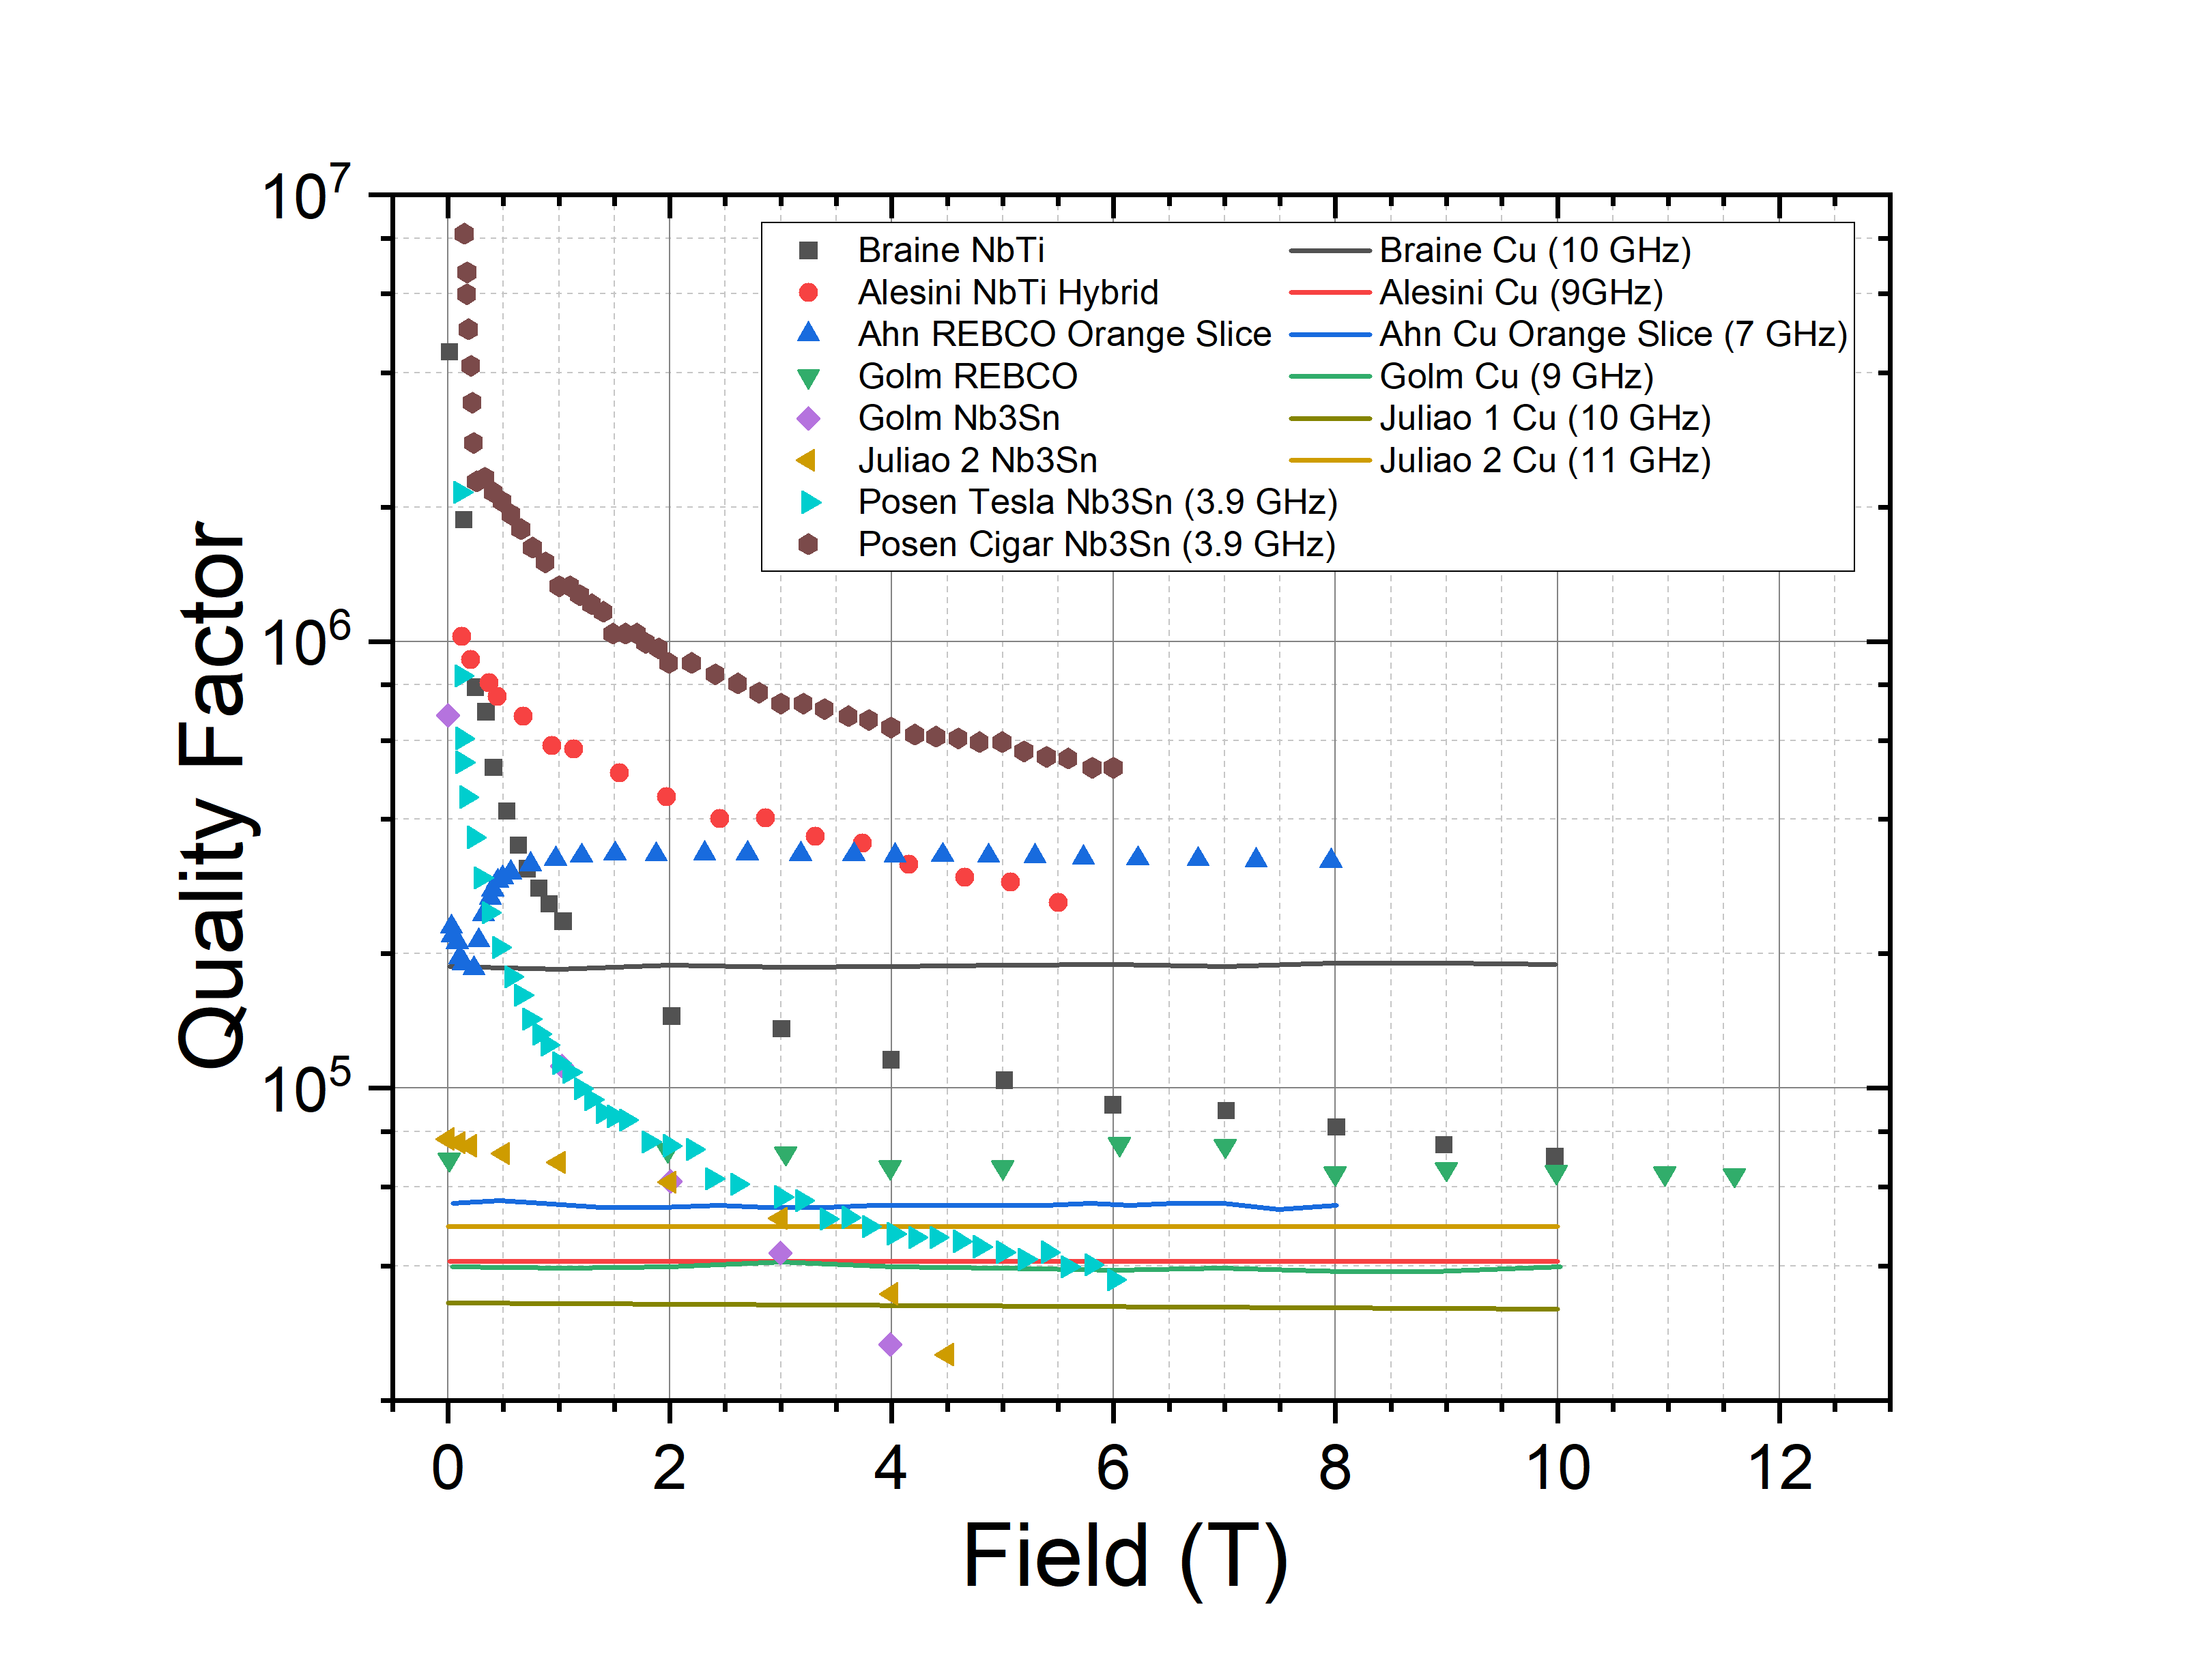
\includegraphics[width=0.9\textwidth]{images/OtherAxionDetector/QvsTAxionPrototypesnew.png}
    \caption{Quality factor vs applied magnetic field for superconducting axion detector cavity prototypes from multiple groups. All non-Posen cavities used a Cu cavity reference of the same geometry~\cite{ahnSuperconductingCavityHigh2020, Braine:2024nzi, posenNb3SnSuperconductingRadiofrequency2022, Golm:2021ooj, Alesini:2019ajt}.}
    \label{fig:axionprototypes}
\end{figure}


\section{Experimental detail}

\subsection{Coupon fabrication}

OFHC Cu substrates were cut into \qtyproduct{7.5 x 7.5}{\milli\meter} coupons, mechanically polished to a mirror finish (SiC 400--1200 grit, diamond slurry 5--\qty{1}{\micro\meter}, colloidal silica \qty{0.05}{\micro\meter}), and ultrasonically cleaned in acetone and IPA. A 500\,nm Ta diffusion barrier was DC-magnetron sputtered at \qty{200}{\degreeCelsius} (10\,mTorr Ar, base pressure $5 \times 10^{-9}$\,Torr) to block Sn migration into the Cu substrate. Cu-Sn alloys (13, 24, 33\,wt.\%\,Sn) were thermally evaporated from alumina-coated tungsten baskets at $\sim 3 \times 10^{-7}$\,Torr to thicknesses of 2--10\,\unit{\micro\meter} in \qty{1}{\micro\meter} steps with 30-minute cooling intervals. Two deposition geometries were used:

\begin{itemize}
    \item \textbf{Cu-Sn-first}: Ta/Cu-Sn deposited, then Nb sputtered on top --- enables hot-bronze reaction.
    \item \textbf{Nb-first}: Ta/Nb deposited, then Cu-Sn evaporated on top --- only post-reaction possible; Cu-Sn removed by APS etching after reaction.
\end{itemize}

Nb was sputtered (250\,W, 8\,mTorr Ar) in three reaction variants: hot-bronze (Nb deposited at \qty{715}{\degreeCelsius}), post-reaction (Nb at \qty{200}{\degreeCelsius} then \qty{715}{\degreeCelsius} anneal), or hot-bronze + post-reaction.

\subsection{Cavity fabrication}

Four two-piece hexagonal Cu cavity bodies were machined from bulk OFHC-101 Cu. Each cavity half is a hexagonal prism (\qty{72}{\milli\meter} height, 12.25\,mm flat-face length, 2\,mm minimum wall thickness, 11\,GHz TM$_{010}$). Cavity halves were hand-polished (SiC 400--1200 grit), etched at LLNL in a standard sequence (soap, HCl, dichromate, antioxidant), and annealed at \qty{250}{\degreeCelsius} for 6\,hours in positive-pressure Ar to improve Cu residual resistivity ratio. Nb$_3$Sn coating was applied at FSU using a modified Recipe 3 (Nb-first, see Sec.~\ref{sec:recipes}): 300\,nm HiPIMS Ta (\qty{800}{\volt}, 50\,\unit{\micro\second} pulse), 500\,nm Nb, 5\,\unit{\micro\meter} Cu-33\,wt.\%\,Sn evaporated in steps, post-reaction at \qty{715}{\degreeCelsius} for 3\,hours, APS etch to remove Cu-Sn. Cavity halves were assembled with four 4-40 stainless steel screws and three alignment pegs.

\subsection{RF measurement}

Coupon $T_c$ was measured by SQUID (Quantum Design MPMS-5, ZFC, 1\,mT applied). Cavity $Q$ was measured by $S_{21}$ transmission using a Keysight PNA VNA (10\,dBm output, 1\,kHz IF bandwidth). Loaded $Q_L$ was extracted from the 3\,dB bandwidth; weak coupling was verified by $<$1\,dB reflection dip, confirming $Q_0 \approx 1.1 \times Q_L$. Temperature-dependent measurements used a Physical Property Measurement System (PPMS, Quantum Design, 2\,K--300\,K) and a $^3$He/$^4$He dilution refrigerator at Lawrence Livermore National Laboratory (LLNL, 50\,mK--300\,mK). Field-dependent measurements used the PPMS at 2\,K, stepping 0--9\,T in 0.5\,T increments with the cavity axis parallel to the field.


\section{Results}

\subsection{Cu-Sn concentration and reaction route optimization}

A survey of Cu-Sn compositions (13, 24, 33\,wt.\%\,Sn) with three reaction routes on Cu/Ta substrates establishes the operating space (Fig.~\ref{fig:Nb3SnCuSubSnconcentration}). Across all compositions, the hot-bronze + post-reaction route achieves the highest $T_c$ and sharpest transitions. Optimal composition is 33\,wt.\%\,Sn, consistent with Nb-substrate results~\cite{Juliao2026nb}. $T_c$ at 13\,wt.\%\,Sn reaches only $\sim$\qty{11}{\kelvin} due to insufficient Sn volume; 24\,wt.\%\,Sn reaches $\sim$\qty{13}{\kelvin}; 33\,wt.\%\,Sn reaches $\sim$\qty{16}{\kelvin}. The \qty{2}{\kelvin} gap between the Nb-substrate optimum (\qty{17.8}{\kelvin}) and the Cu optimum (\qty{16}{\kelvin}) is attributed to CTE compressive strain~\cite{ekinStrainScalingLaw1980}.

\begin{figure}[htb]
    \centering
    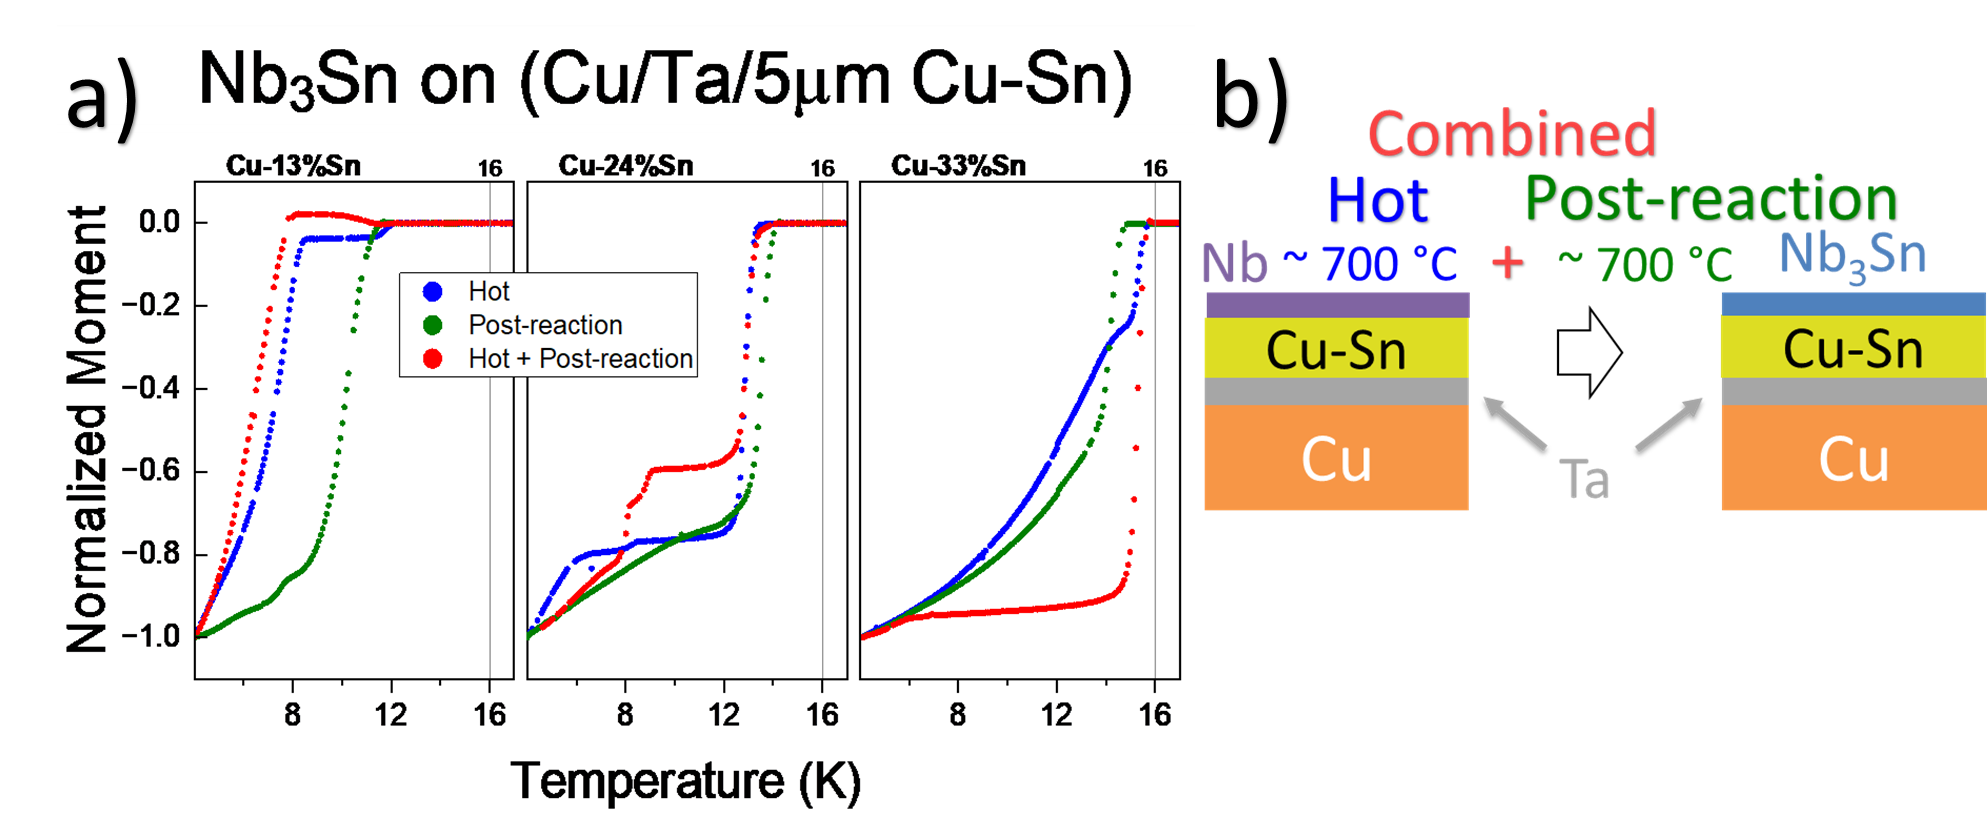
\includegraphics[width=0.9\textwidth]{images/Cu/Nb3SnCuSubSnconcentration.png}
    \caption{(a) $T_c$ curves for Nb$_3$Sn on Cu/Ta substrates with varying Cu-Sn composition and reaction route. (b) Multilayer schematic. Hot-bronze + post-reaction with 33\,wt.\%\,Sn achieves the highest $T_c$ and sharpest transition.}
    \label{fig:Nb3SnCuSubSnconcentration}
\end{figure}

\subsection{Three optimized recipes}\label{sec:recipes}

From the systematic study, three recipes were selected for distinct advantages (Fig.~\ref{fig:Recipe123Tc}):

\begin{figure}[htb]
    \centering
    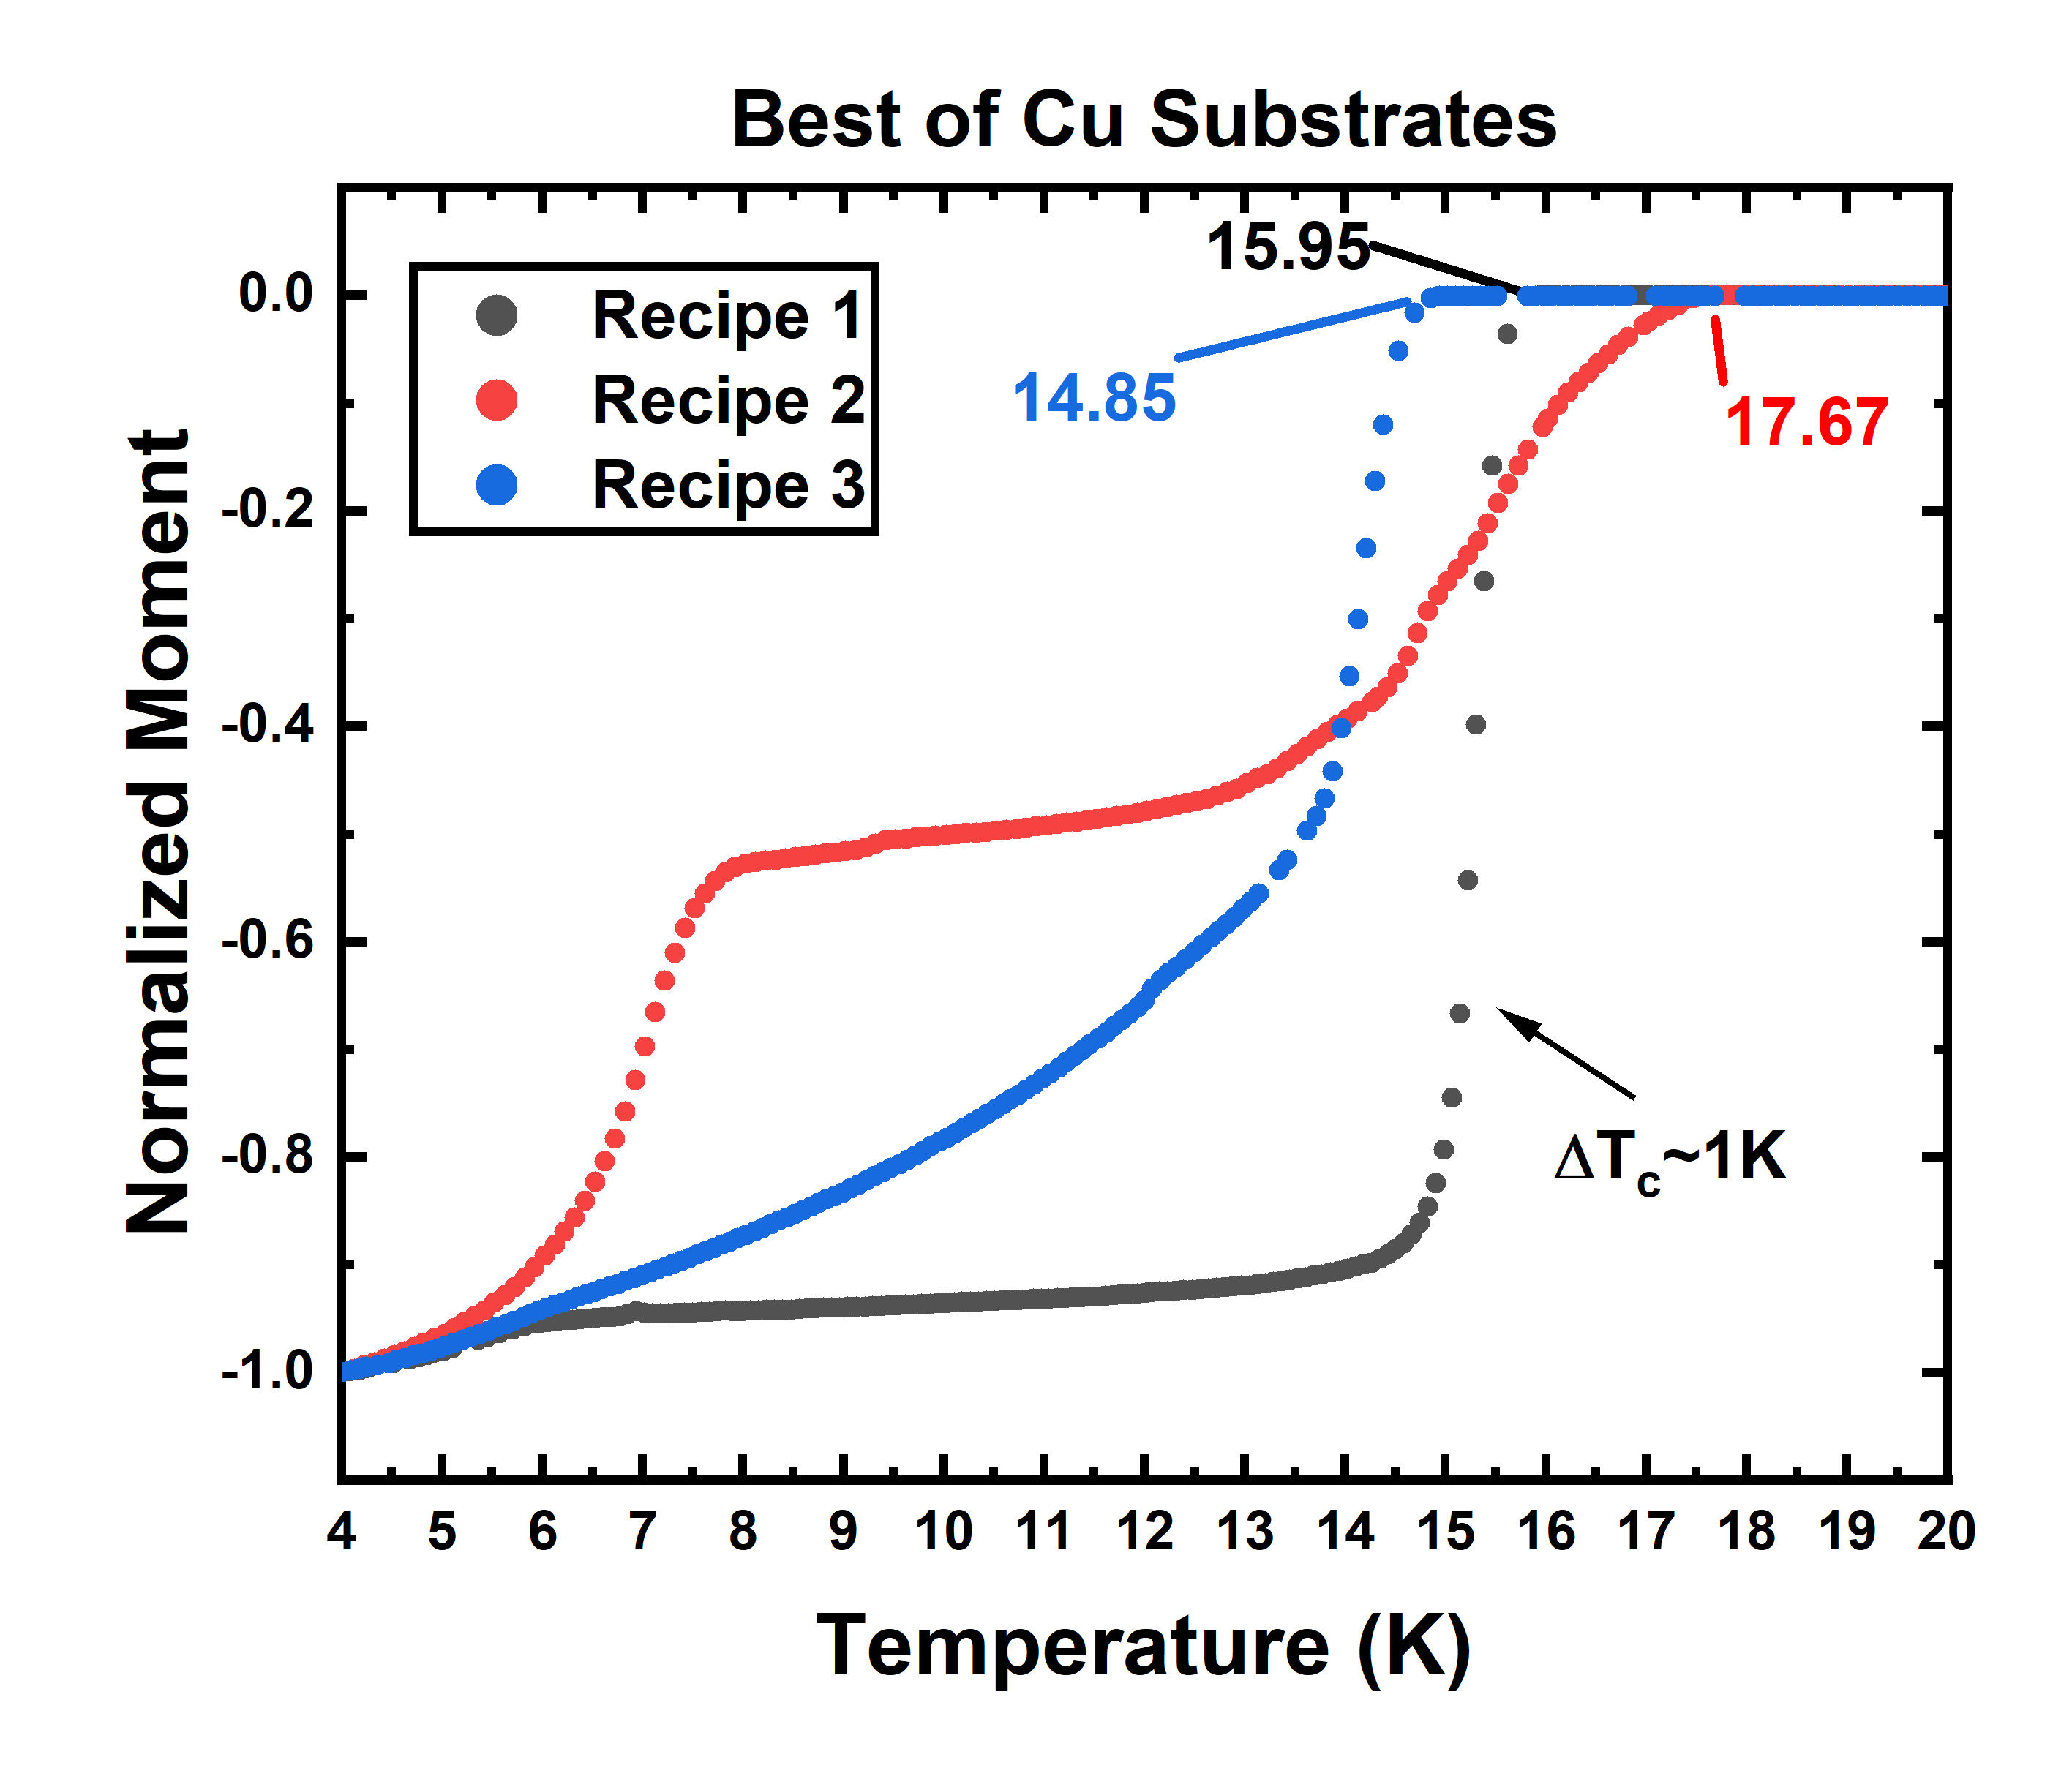
\includegraphics[width=0.7\textwidth]{images/Cu/Recipe123Tc.png}
    \caption{$T_c$ curves for the three optimized Cu-substrate recipes. Recipe 1 (black): thin Cu-Sn first, $\Delta T_c < \qty{1}{\kelvin}$. Recipe 2 (red): thick Cu-Sn first, $T_c = \qty{17.7}{\kelvin}$. Recipe 3 (blue): Nb-first, superior morphological uniformity.}
    \label{fig:Recipe123Tc}
\end{figure}

\subsubsection{Recipe 1: Thin Cu-Sn first (hot-bronze + post-reaction)}

A 500\,nm Ta barrier, 5\,\unit{\micro\meter} Cu-33\,wt.\%\,Sn, 300\,nm Nb deposited at \qty{700}{\degreeCelsius}, followed by 3-hour post-reaction. This sample achieved $T_c = \qty{16}{\kelvin}$ and $\Delta T_c < \qty{1}{\kelvin}$ (Fig.~\ref{fig:Recipe123Tc}, black), the sharpest transition obtained among Cu-compatible routes in this work and competitive with literature~\cite{fonnesuRecipeOptimizationSRF2025, luImpactCuSn2025}. Cross-sectional SEM (Fig.~\ref{fig:300nmNb3sn16K}) shows the multilayer structure; delamination in the Cu-Sn layer is consistent with Ta-barrier samples under CTE stress. The EDS linescan confirms $\sim$25\,at.\%\,Sn throughout the Nb$_3$Sn thickness (Fig.~\ref{fig:FullNb3Sn10micron}).

\begin{figure}[htb]
    \centering
    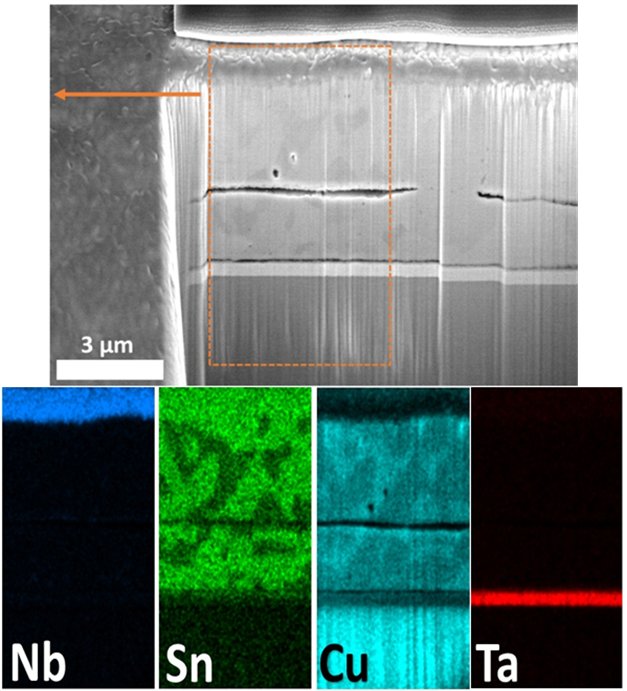
\includegraphics[width=0.55\textwidth]{images/Cu/300nmNb3sn16K.png}
    \caption{Recipe 1 cross-section: Cu/Ta/Cu-Sn/Nb$_3$Sn multilayer. Delamination in the Cu-Sn layer is attributed to CTE mismatch stress at the Ta interface.}
    \label{fig:300nmNb3sn16K}
\end{figure}

\begin{figure}[htb]
    \centering
    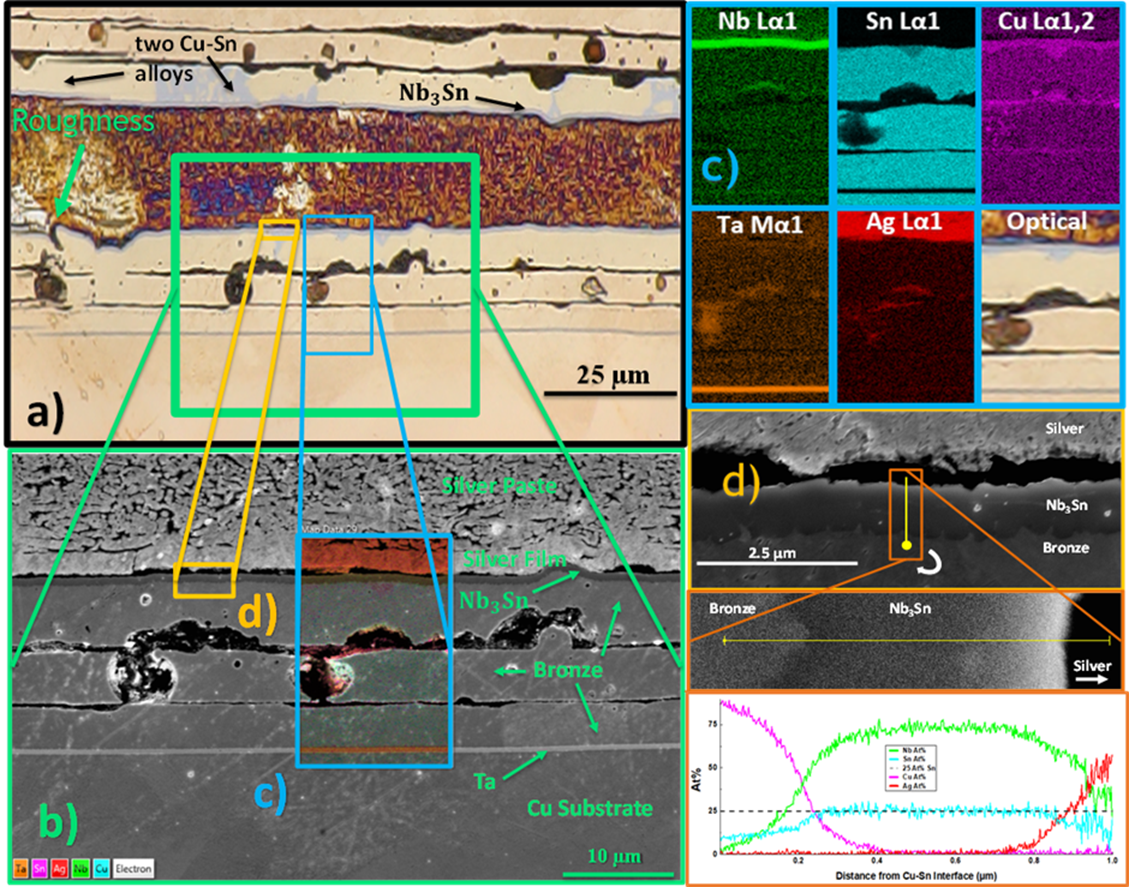
\includegraphics[width=0.9\textwidth]{images/Cu/CuSnThickness/FullNb3Sn10micron.png}
    \caption{Full cross-sectional characterization of a Cu-Sn-first film: (a) optical micrograph, (b) SEM, (c) EDS maps (Nb, Sn, Cu, Ta), and (d) EDS linescan confirming $\sim$25\,at.\%\,Sn uniformly across the Nb$_3$Sn thickness. The EDS map reveals that Sn penetrated through the Ta barrier into the Cu substrate.}
    \label{fig:FullNb3Sn10micron}
\end{figure}

\subsubsection{Recipe 2: Thick Cu-Sn first (hot-bronze)}

A 500\,nm Nb diffusion barrier, 5\,\unit{\micro\meter} Cu-33\,wt.\%\,Sn, 3\,\unit{\micro\meter} Nb deposited at \qty{700}{\degreeCelsius}, no post-reaction. This film achieved $T_c = \qty{17.7}{\kelvin}$ (Fig.~\ref{fig:Recipe123Tc}, red), approaching the Nb-substrate maximum. The high $T_c$ onset is attributed to partial CTE strain relaxation in the thicker Nb$_3$Sn film~\cite{Ilyina-Brunner:2019iay}. However, the broad transition ($\Delta T_c \sim 3$\,K) reflects Sn depletion at the surface of the thick film due to limited Sn supply volume. Cross-section (Fig.~\ref{fig:Thicknb3sn17K}) shows no delamination, consistent with the Nb diffusion barrier allowing more compliant CTE accommodation.

\begin{figure}[htb]
    \centering
    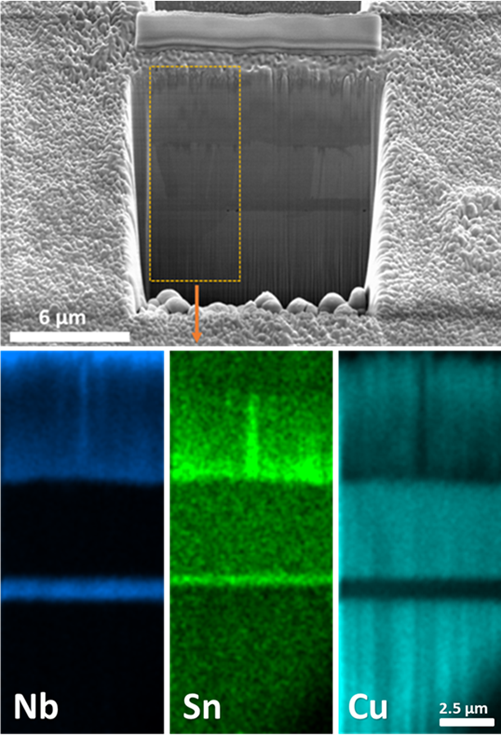
\includegraphics[width=0.55\textwidth]{images/Cu/Thicknb3sn17K.png}
    \caption{Recipe 2 cross-section: Cu/Nb barrier/Cu-Sn/3\,\unit{\micro\meter} Nb$_3$Sn. No delamination in the Cu-Sn layer. Broad $T_c$ transition reflects Sn depletion across the thick film.}
    \label{fig:Thicknb3sn17K}
\end{figure}

\subsubsection{Recipe 3: Nb-first (post-reaction + etch)}

A 500\,nm Ta barrier, 500\,nm Nb, 5\,\unit{\micro\meter} Cu-33\,wt.\%\,Sn evaporated on top, post-reaction at \qty{715}{\degreeCelsius} for 3\,hours, Cu-Sn removed by APS etching. This route cannot use hot-bronze (Cu-Sn arrives after Nb), but produces exceptionally uniform Nb$_3$Sn morphology because Ta and Nb are deposited sequentially in vacuum with a sharp, clean interface (Fig.~\ref{fig:BronzeOnNb}). The $T_c$ onset is $\sim$\qty{15}{\kelvin} with broader $\Delta T_c \sim 2$\,K due to incomplete reaction (time-constrained), but the lateral uniformity is superior to Cu-Sn-first routes. Recipe 3 was selected for cavity coating. A three-route $T_c$ comparison (Fig.~\ref{fig:ReactionComparisonwith}) confirms the trade-off: hot-bronze + post-reaction gives the sharpest transition; Nb-first gives the most uniform morphology.

\begin{figure}[htb]
    \centering
    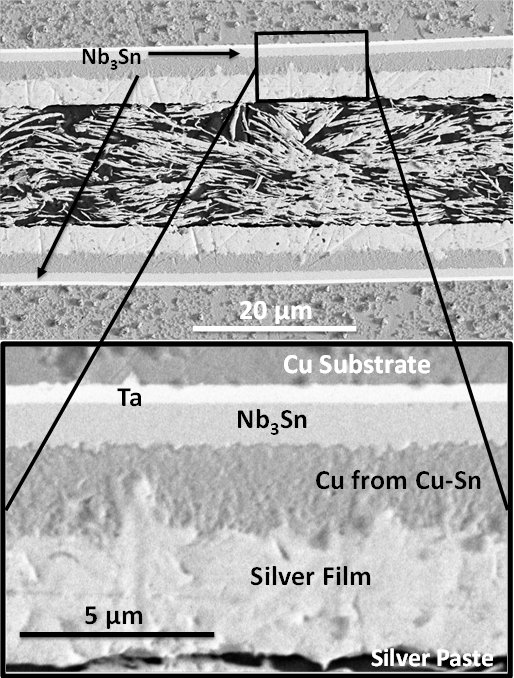
\includegraphics[width=0.55\textwidth]{images/Cu/BronzeOnNb/BronzeOnNb.png}
    \caption{Recipe 3 cross-section: exceptionally uniform Nb$_3$Sn film resulting from the sharp Ta/Nb interface formed by sequential in-vacuum sputtering.}
    \label{fig:BronzeOnNb}
\end{figure}

\begin{figure}[htb]
    \centering
    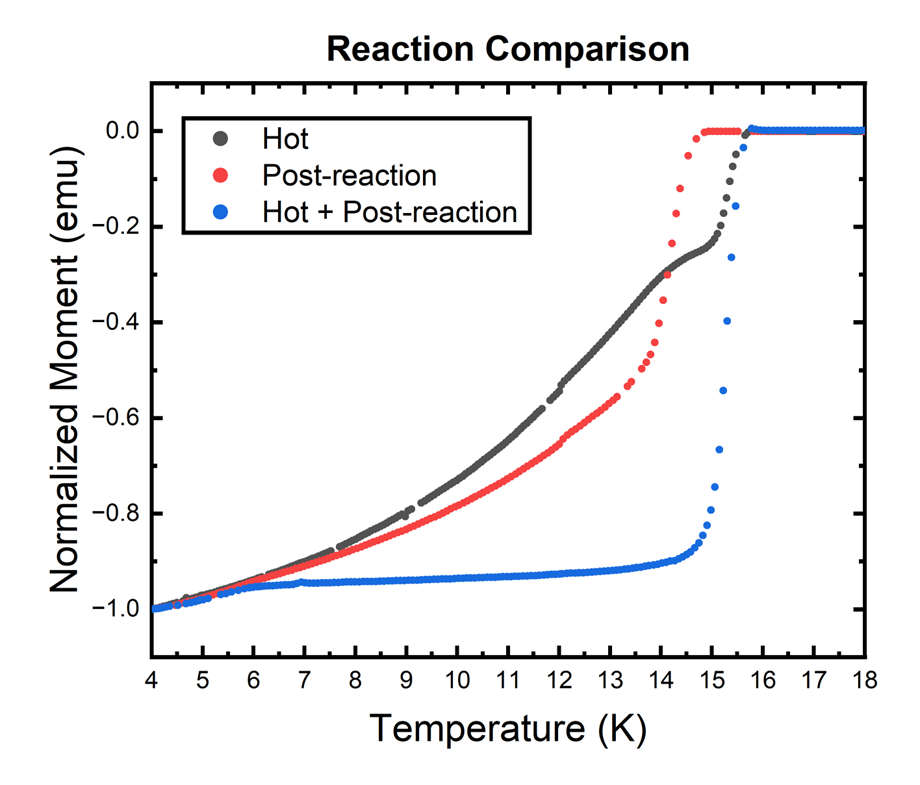
\includegraphics[width=0.7\textwidth]{images/Cu/ReactionComparisonwith.png}
    \caption{$T_c$ comparison of three Cu/Ta substrate processing routes. Hot-bronze + post-reaction (Recipe 1, blue) achieves the sharpest transition ($\Delta T_c \sim \qty{1}{\kelvin}$); Nb-first (Recipe 3, red) is broader but morphologically superior.}
    \label{fig:ReactionComparisonwith}
\end{figure}

\subsection{Cavity design: hexagonal geometry}

The two-piece hexagonal prism geometry was chosen over a cylinder for two reasons. First, it fits within the deposition system clearance (13\,mm max thickness, Fig.~\ref{fig:ClearenceSputter}). Second, COMSOL simulations (Fig.~\ref{fig:GapnoGapCylinderHexagon}) showed that locating the two assembly seams at the hexagon corners reduces seam-related $Q$ degradation from $\sim$27\% (cylinder) to $\sim$1\% (hexagon), because RF surface currents are concentrated at the face centers and minimized at corners.

\begin{figure}[htb]
    \centering
    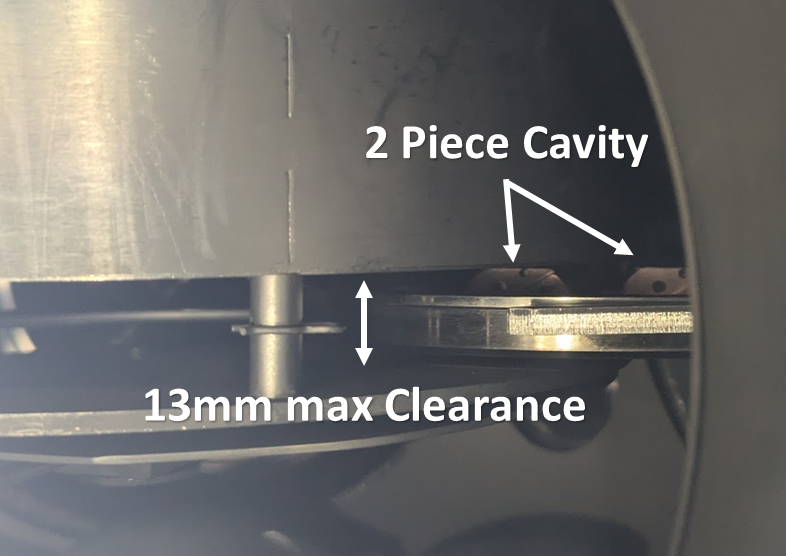
\includegraphics[width=0.75\linewidth]{images/AndreCavity/ClearenceSputter.png}
    \caption{Sputtering chamber geometry constraining cavity piece thickness to $\leq 13$\,mm.}
    \label{fig:ClearenceSputter}
\end{figure}

\begin{figure}[htb]
    \centering
    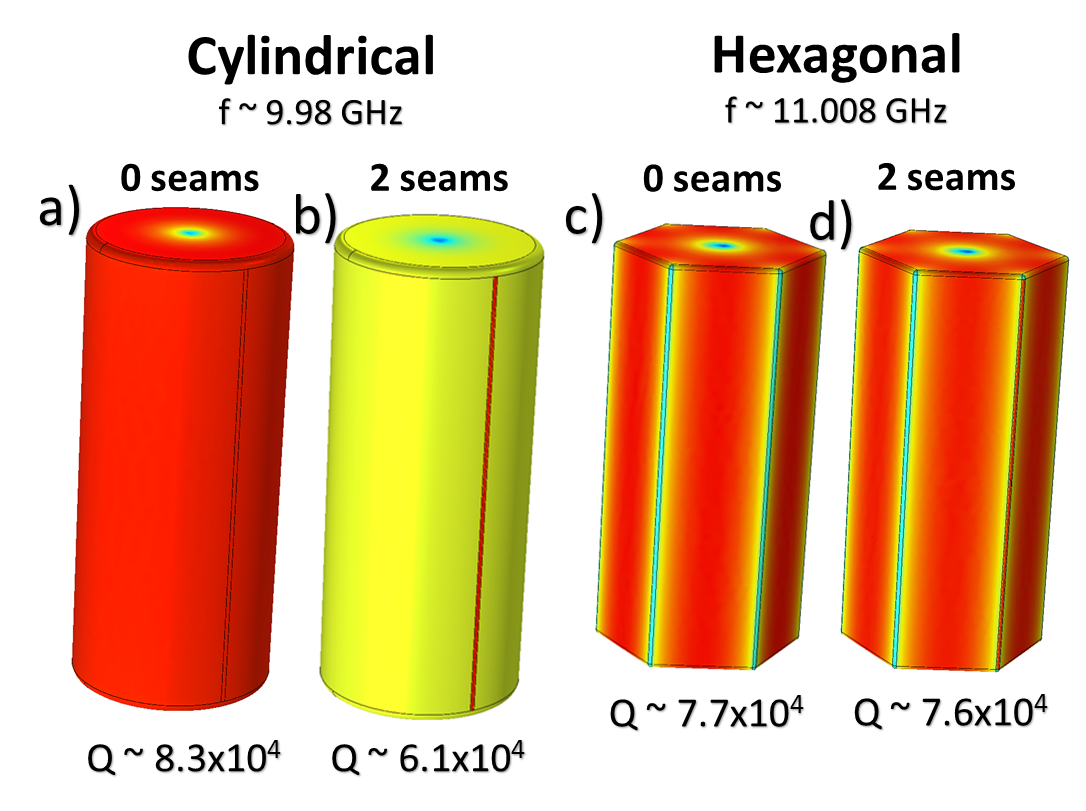
\includegraphics[width=0.85\linewidth]{images/AndreCavity/GapnoGapCylinderHexagon.png}
    \caption{COMSOL simulations of cylinder (a, b) and hexagonal (c, d) cavity geometries, with and without a resistive seam. Color scale: surface current (red = max, green = min). Adding a seam at the wall reduces cylinder $Q$ by $\sim$27\% but hexagon $Q$ by only $\sim$1\%.}
    \label{fig:GapnoGapCylinderHexagon}
\end{figure}

\subsection{RF results: Cu cavity baseline}

The bare Cu cavity (2-piece, assembled) was characterized as a reference at each processing stage (Fig.~\ref{fig:CuCavitiesRsvsT}). Initial hand-polished assembly: $Q = 12{,}000$ (RT), $Q = 35{,}000$ (4\,K). After LLNL etch: $Q = 49{,}000$ (4\,K). After 250\,\unit{\degreeCelsius} 6-hr Ar anneal: $Q = 55{,}000$ (4\,K), approaching the COMSOL ideal of $Q = 76{,}000$ for seamless RRR-300 Cu at 11\,GHz. The residual gap ($55{,}000$ vs $76{,}000$) is attributed to RF leakage at the mechanical seam.

\begin{figure}[htb]
    \centering
    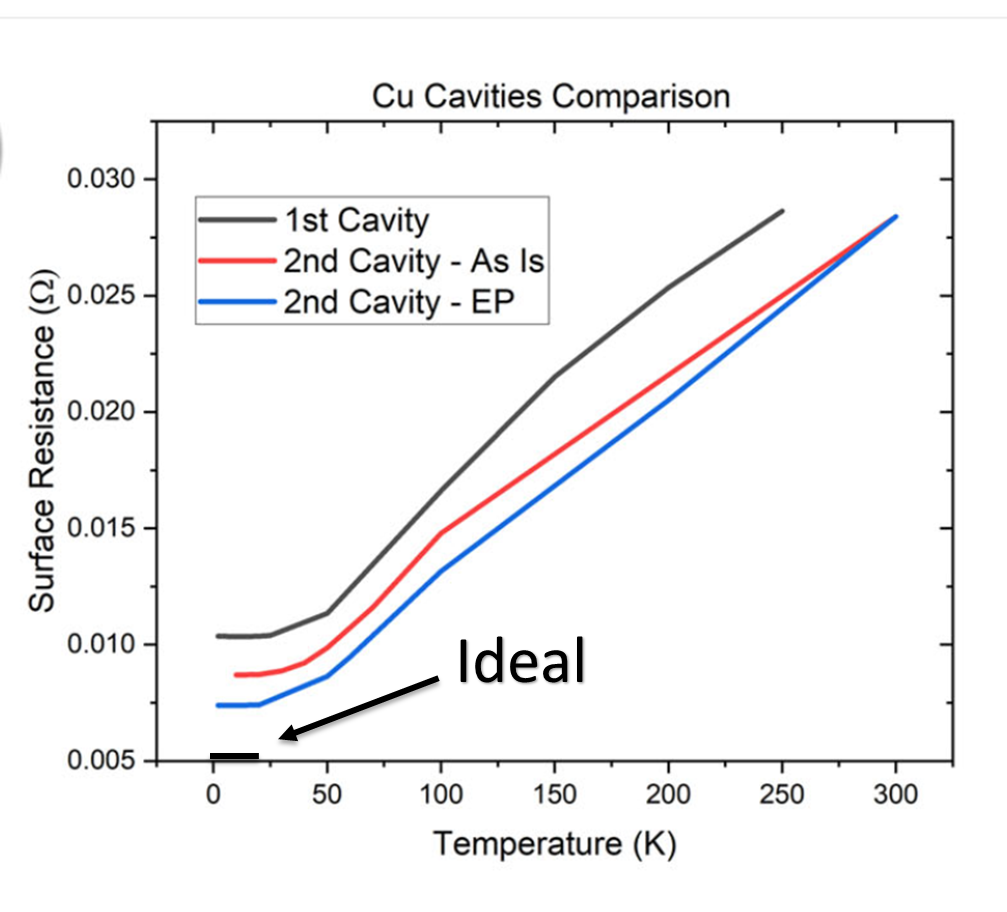
\includegraphics[width=0.7\linewidth]{images/AndreCavity/CuCavitiesRsvsT.png}
    \caption{Surface resistance vs temperature for the 8-piece prototype (1st cavity) and 2-piece cavity at successive processing stages. The ideal 5\,m$\Omega$ line corresponds to COMSOL-simulated RRR-300 Cu at 11\,GHz.}
    \label{fig:CuCavitiesRsvsT}
\end{figure}

\subsection{RF results: Nb$_3$Sn-coated cavity at ASC and LLNL}

The fully coated 2-piece Nb$_3$Sn cavity was measured in the PPMS (2\,K--300\,K, zero field) and in the LLNL dilution refrigerator (50\,mK--300\,mK, zero field). Results are shown in Figs.~\ref{fig:2pieceCavityResults} and~\ref{fig:LLNLDilutionQtest}. The loaded quality factor was constant at $Q_L = 77{,}000$ ($R_s = 5$\,m$\Omega$) from 50\,mK to 300\,mK, and $Q_L = 59{,}000$ ($R_s = 6$\,m$\Omega$) at 2\,K. Unloaded values are approximately 10\% higher: $Q_0 \approx 85{,}000$ at 50\,mK and $Q_0 \approx 65{,}000$ at 2\,K.

\begin{figure}[htb]
    \centering
    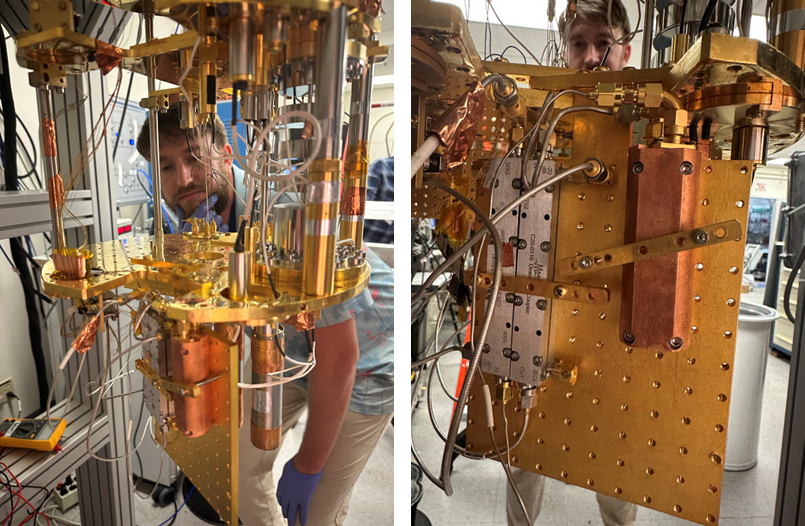
\includegraphics[width=0.7\linewidth]{images/AndreCavity/LLNLDilutionQtest.png}
    \caption{LLNL dilution refrigerator setup for 50\,mK $Q$ measurements.}
    \label{fig:LLNLDilutionQtest}
\end{figure}

\begin{figure}[htb]
    \centering
    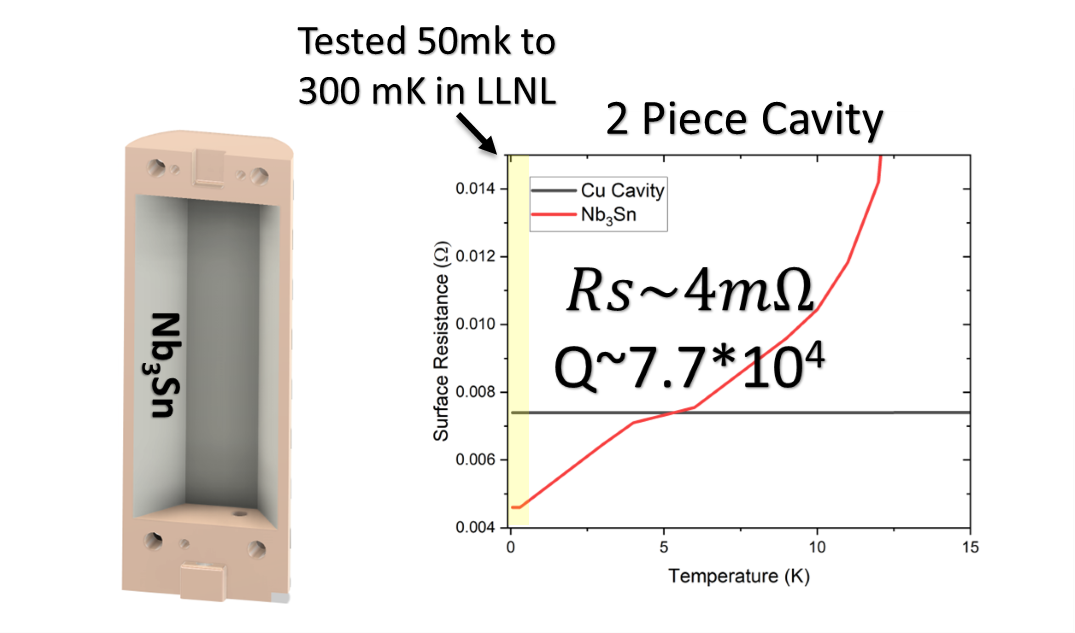
\includegraphics[width=0.9\linewidth]{images/AndreCavity/2pieceCavityResults.png}
    \caption{Model and surface resistance vs temperature for the 2-piece Nb$_3$Sn-coated cavity. $Q_L = 77{,}000$ at 50\,mK, $Q_L = 59{,}000$ at 2\,K.}
    \label{fig:2pieceCavityResults}
\end{figure}

\subsection{Corrections to quality factor}

Visual inspection after measurement revealed that both endcaps lost their Nb$_3$Sn coating during APS etching (Fig.~\ref{fig:EdgeEffect2piece}), leaving $\sim$1/3 of the cavity surface as bare Cu. To estimate the performance of a fully coated cavity with no seam losses, two corrections were applied:

\textbf{Correction 1 --- Cu endcaps.} For a hybrid cavity with geometric factor $G_\text{total} = 350\,\Omega$, split as $G_\text{Cu} = 1050\,\Omega$ (1/3 surface) and $G_\text{Nb$_3$Sn} = 525\,\Omega$ (2/3 surface):
\begin{equation}
    \frac{1}{Q_\text{meas}} = \frac{R_{s,\text{Cu}}}{G_\text{Cu}} + \frac{R_{s,\text{Nb$_3$Sn}}}{G_\text{Nb$_3$Sn}}
\end{equation}
Using $R_{s,\text{Cu}} = 6.36$\,m$\Omega$ (measured Cu cavity at 50\,mK), solving for $R_{s,\text{Nb$_3$Sn}} = 3.64$\,m$\Omega$ gives:
\begin{equation}
    Q_\text{Nb$_3$Sn,full} = G_\text{total}/R_{s,\text{Nb$_3$Sn}} = 350/3.64\times10^{-3} = 9.6\times10^4
\end{equation}

\textbf{Correction 2 --- RF seam leakage.} The measured Cu cavity ($Q = 55{,}000$) fell below the ideal seamless simulation ($Q = 76{,}000$), giving a correction factor $\alpha = 76{,}000/55{,}000 = 1.38$. Applying to the Nb$_3$Sn result:
\begin{equation}
    Q_\text{Nb$_3$Sn,corrected} = 1.38 \times 9.6\times10^4 = 1.3\times10^5
\end{equation}
With the 10\% unloaded correction: $Q_{0,\text{corrected}} \approx 1.4 \times 10^5$ at 50\,mK, zero field.

\begin{figure}[htb]
    \centering
    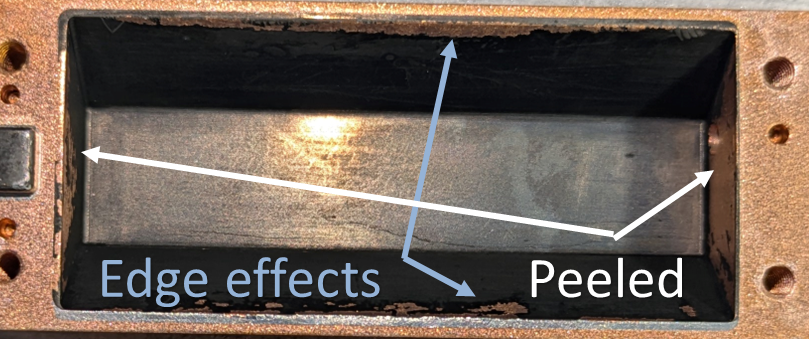
\includegraphics[width=0.75\linewidth]{images/AndreCavity/EdgeEffect2piece.png}
    \caption{Coating defects at endcap regions after APS etching: Nb$_3$Sn delaminated from both endcaps, leaving $\sim$1/3 of the cavity surface as bare Cu. Line-of-sight deposition did not effectively coat surfaces perpendicular to the deposition flux.}
    \label{fig:EdgeEffect2piece}
\end{figure}


\subsection{Quality factor vs magnetic field}

Field-dependent $Q$ was measured on the 8-piece prototype cavity (one Nb$_3$Sn wall, Cu endcaps and remaining 5 walls) at 2\,K in the PPMS (Fig.~\ref{fig:8pieceQvsB}). $Q$ degraded linearly with field and superconductivity was lost at $\sim$8\,T, far below the expected $H_{c2} > 20$\,T for Nb$_3$Sn wires. At low field ($B < 1$\,T), the superconducting wall was more resistive than bare Cu. This anomalous behavior is attributed to the CTE-induced compressive strain lowering the vortex entry field ($H_\text{entry} \approx 11.4$\,mT~\cite{luImpactCuSn2025}): vortices penetrate at very low fields, and their oscillation under RF dissipates energy via Campbell resistance. Film roughness ($\sim$500\,nm scale) also produces surface field components perpendicular to the external field, generating large Lorentz forces on vortices even when the wall is nominally parallel to the field.

\begin{figure}[htb]
    \centering
    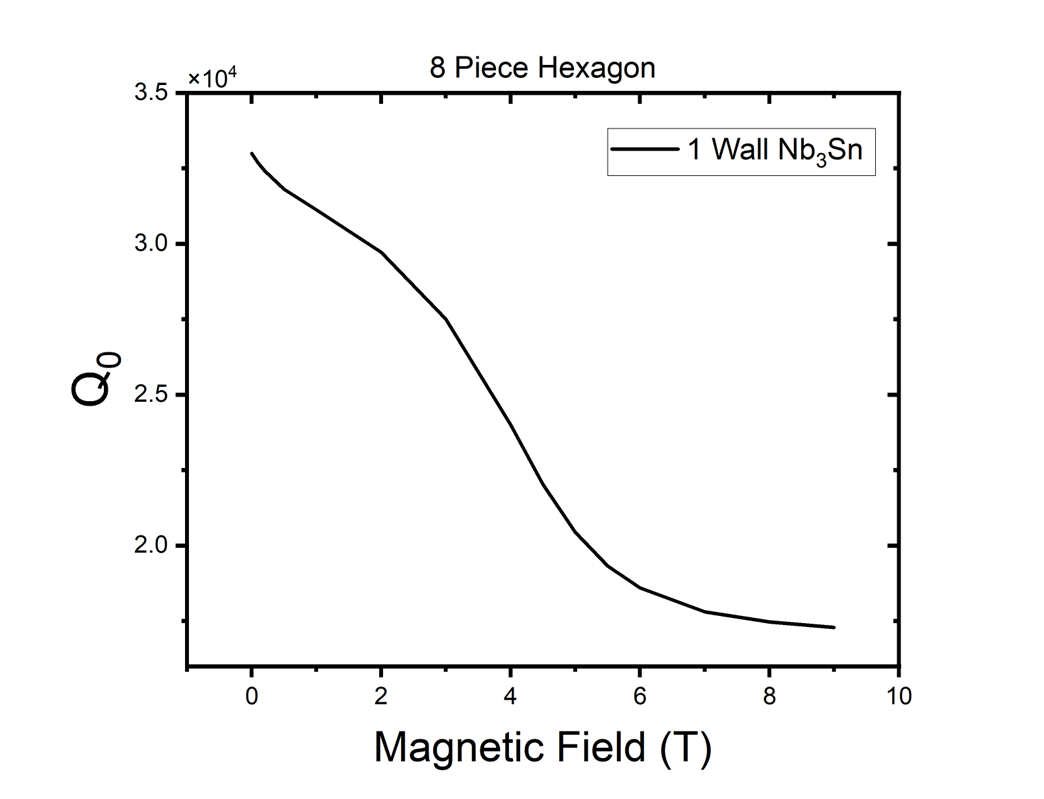
\includegraphics[width=0.75\linewidth]{images/AndreCavity/8pieceQvsB.png}
    \caption{Quality factor vs magnetic field at 2\,K for the 8-piece prototype cavity with one Nb$_3$Sn wall. Superconductivity is lost at $\sim$8\,T, far below the bulk $H_{c2}$. Linear $Q$ degradation with field is consistent with Campbell resistance from CTE strain-driven low vortex entry field.}
    \label{fig:8pieceQvsB}
\end{figure}

\section{Discussion}

\subsection{Film optimization: comparing three recipes}

The three recipes reveal a clear performance--uniformity trade-off on Cu substrates. Recipe 1 achieves the best stoichiometric uniformity ($\Delta T_c < 1$\,K) through the two-step hot-bronze + post-reaction process, which first establishes the Nb$_3$Sn microstructure during hot deposition and then homogenizes Sn distribution in a follow-up anneal. Recipe 2 demonstrates that $T_c$ on Cu can approach the Nb-substrate maximum when film thickness is sufficient for strain relaxation, at the cost of stoichiometric uniformity in thick films with limited Sn supply. Recipe 3's superior lateral uniformity, resulting from the clean Ta/Nb interface, outweighs its lower $T_c$ for the cavity application: RF surface resistance is primarily limited by lateral non-uniformity (areas of low-Sn or missing Nb$_3$Sn), not by the mean $T_c$.

\subsection{Cavity performance and comparison with competing groups}

The corrected $Q_0 \approx 1.4 \times 10^5$ at 50\,mK, zero field represents a factor $\sim$2.5$\times$ improvement over the bare Cu reference ($Q = 55{,}000$). Compared to the axion detector landscape (Fig.~\ref{fig:axionprototypes}), this zero-field result is comparable to the best NbTi bulk cavity ($Q \sim 10^6$ at zero, but drops to $7.5 \times 10^4$ at 9\,T) and exceeds most thin-film NbTi results. The CAPP REBCO cavity ($Q \sim 3 \times 10^5$ at 9\,T) currently leads at high field due to REBCO's $H_{c2} > 100$\,T. The primary challenge for Nb$_3$Sn on Cu is maintaining high $Q$ in applied field: CTE-induced compressive strain lowers the vortex entry field ($H_\text{entry} \approx 11.4$\,mT~\cite{luImpactCuSn2025}), causing rapid vortex penetration and $Q$ degradation with increasing $B$.

\subsection{Pathways for improvement}

The key obstacle to high-field performance is the CTE mismatch strain. Strategies to mitigate it include: (1) thick Nb buffer layers ($\geq 30$\,\unit{\micro\meter}) to relax strain before Nb$_3$Sn formation~\cite{Ilyina-Brunner:2019iay}; (2) intermediate substrates with CTE closer to Nb$_3$Sn (e.g., sapphire inserts on Cu); and (3) multilayer thin-film architectures where the Nb$_3$Sn layer is decoupled from the Cu substrate stress. Endcap coating uniformity, the most immediate loss mechanism identified, can be addressed by tilted deposition geometry or rotating substrate fixtures.


\section{Conclusions}

Three Cu-compatible Nb$_3$Sn recipes were developed and down-selected to Recipe 3 (Nb-first) for cavity coating based on morphological uniformity. A two-piece hexagonal Cu cavity coated with Recipe 3 achieved $Q_L = 77{,}000$ at 50\,mK, zero field, measured in a dilution refrigerator at LLNL. After correcting for uncoated Cu endcaps and RF seam leakage, the estimated quality factor for a fully coated, seam-free Nb$_3$Sn cavity is $Q_0 \approx 1.4 \times 10^5$. This is the first demonstration of a Nb$_3$Sn-coated RF cavity fabricated on a copper substrate using the Cu-Sn ternary bronze route. The primary path to further improvement is reducing CTE-induced compressive strain, which currently limits the vortex entry field and causes rapid $Q$ degradation in applied magnetic fields relevant to axion dark matter searches.

\ack
This work was supported in part by a DOE Office of Science Graduate Student Research (SCGSR) fellowship, with collaboration from Dr. G. Carosi and the LLNL team. Work at the Applied Superconductivity Center was supported by [funding source TBD].

\section*{Author contributions}
A.R.J. fabricated samples, performed measurements, designed and built the cavity, and wrote the manuscript. L.D.C. supervised the project and edited the manuscript.

\section*{Data availability statement}
Data supporting this study are available from the corresponding author upon reasonable request.

\printbibliography

\end{document}
